% Reporte de la actividad 6A — Agrupamiento, análisis de tópicos y visualización de un corpus
% Compilación: latexmk -pdf -jobname=Reporte_Actividad6A reporte.tex
% Las cifras provienen de results/*.csv y las figuras de figures/ (generadas por el notebook).
% Límite de la actividad: máximo tres páginas.
\documentclass[10pt,a4paper]{article}

\usepackage[T1]{fontenc}
\usepackage[utf8]{inputenc}
\usepackage[spanish,es-nodecimaldot]{babel}
\usepackage[margin=1.6cm,top=1.4cm,bottom=1.5cm]{geometry}
\usepackage{amsmath}
\usepackage{booktabs}
\usepackage{array}
\usepackage{xcolor}
\usepackage{microtype}
\usepackage{enumitem}
\usepackage{graphicx}
\usepackage{float}
\usepackage[font=small,labelfont=bf,skip=2pt]{caption}
\usepackage[hidelinks]{hyperref}

\graphicspath{{figures/}}

\definecolor{acento}{HTML}{1F6FEB}
\newcommand{\term}[1]{\textcolor{acento}{\emph{#1}}}

\setlist[itemize]{topsep=1pt,itemsep=0pt,parsep=0pt,leftmargin=1.2em}
\setlength{\parskip}{2pt}
\setlength{\textfloatsep}{5pt}
\setlength{\floatsep}{5pt}
\setlength{\intextsep}{4pt}
\renewcommand{\arraystretch}{1.0}
\usepackage{titlesec}
\titlespacing*{\section}{0pt}{4pt}{1pt}
\titlespacing*{\paragraph}{0pt}{2pt}{0.6em}

\title{\vspace{-1.5cm}\textbf{Agrupamiento, tópicos y visualización de un corpus sin etiquetas}\\[2pt]
\large Qué estructura encuentra el método por sí solo, cómo se la explica a un lector y qué deforma el mapa}
\author{David Segundo García}
\date{\vspace{-0.3cm}Actividad 6A \textperiodcentered\ 16 de noviembre de 2026
\textperiodcentered\ acompaña al notebook \texttt{Actividad6A\_Agrupamiento\_Topicos.ipynb}}

\begin{document}
\maketitle
\vspace{-0.95cm}

\section{Flujo de trabajo y representación}

\paragraph{Escenario.} Se toman los \textbf{120 documentos en español} de las unidades 2 y 4 (título + cuerpo,
45--81 palabras). Su categoría editorial se \textbf{aparta en la primera celda} y ninguna decisión la usa:
solo vuelve en la sección~5 como auditoría. El flujo es
\emph{embeddings} $\rightarrow$ agrupamiento (3 estrategias, silueta) $\rightarrow$ tópicos (c-TF-IDF)
$\rightarrow$ mapa UMAP con interfaz \texttt{ipywidgets}.

\paragraph{¿Sirve para agrupar la mejor representación para recuperar?} Se compararon cuatro representaciones
densas normalizadas. Dos se reutilizaron de la unidad~4: \textbf{MiniLM} (384\,d) y \textbf{E5} con prefijo
\texttt{passage:}, el mejor \emph{bi-encoder} de la 4A. Dos se generaron nuevas: \textbf{E5} con prefijo
\texttt{query:}, que su ficha recomienda para tareas simétricas, y \textbf{mpnet}
(\texttt{paraphrase-multilingual-mpnet-base-v2}, 768\,d). El criterio, interno y sin etiquetas, fue la
\textbf{silueta coseno de K-Means}, promediada en la meseta $6\le k\le 20$ para no depender de un solo $k$.

\begin{table}[H]
\centering\footnotesize\setlength{\tabcolsep}{5pt}
\begin{tabular}{@{}llrccc@{}}
\toprule
\textbf{Representación} & \textbf{Origen} & \textbf{Dim.} & \textbf{Coseno medio [mín, máx]} & \textbf{Silueta media ($k$ 6--20)} & \textbf{Silueta máx. ($k$)} \\
\midrule
mpnet (paráfrasis)        & nuevo     & 768 & 0.19 [$-$0.14, 0.75] & \textbf{0.160} & \textbf{0.177} (12) \\
MiniLM (paráfrasis)       & unidad 4  & 384 & 0.20 [$-$0.17, 0.80] & 0.145 & 0.166 (14) \\
E5 + \texttt{query:}      & nuevo     & 768 & 0.82 [0.76, 0.90]    & 0.059 & 0.066 (12) \\
E5 + \texttt{passage:}    & unidad 4  & 768 & 0.77 [0.69, 0.89]    & 0.058 & 0.066 (13) \\
\bottomrule
\end{tabular}
\end{table}

\textbf{No.} E5, el mejor modelo para buscar en la 4A, es el peor para agrupar. Hay dos razones con evidencia.
(1) \textbf{Anisotropía}: todos sus cosenos caen en una banda estrecha y alta, así que la distancia
intra-grupo apenas difiere de la inter-grupo. (2) \textbf{Objetivo de entrenamiento}: E5 aprendió a
emparejar consultas cortas con pasajes (tarea asimétrica), mientras que los modelos de paráfrasis aprendieron
justo lo que pide agrupar, que es comparar pasaje con pasaje. Centrar E5 restando el vector medio corrige la
anisotropía (coseno medio $-$0.01), pero la silueta solo sube de 0.058 a 0.070. El prefijo \texttt{query:}
tampoco ayuda. Se eligió \textbf{mpnet}: la auditoría posterior confirmó el mismo orden (ARI a $k=12$:
mpnet 0.59, MiniLM 0.50, E5 0.48 y 0.44).

\section{Estructura oculta: tres estrategias y una regla de selección}

Se compararon tres familias con supuestos distintos sobre mpnet. \textbf{K-Means} supone grupos convexos de
tamaño parecido; \textbf{aglomerativo Ward} supone una estructura jerárquica; \textbf{UMAP 5D + HDBSCAN}
(el esquema de BERTopic) busca regiones densas de forma libre y admite ruido. En las dos primeras se varió
$k=2\ldots20$; en la tercera, \texttt{n\_neighbors} $\in\{10,15\}$ y \texttt{min\_cluster\_size} $\in\{3\ldots8\}$.
La \textbf{regla se fijó antes de ver resultados}:
\begin{itemize}
\item \textbf{Silueta coseno en el espacio original}, también para HDBSCAN: medirla en el espacio de UMAP
la inflaría. Cada documento marcado como ruido aporta silueta 0. Al excluirlo, la de HDBSCAN subía de 0.180 a
0.200 y habría ganado solo por descartar los documentos difíciles.
\item Restricción de utilidad: ningún grupo con menos de \textbf{5 documentos} y $\le$\textbf{10\,\%} de ruido.
\item Respaldo: Davies-Bouldin (DB, menor es mejor) y \textbf{estabilidad} (ARI entre la partición y 20
réplicas con el 80\,\% de los documentos).
\end{itemize}

\begin{figure}[H]
\centering
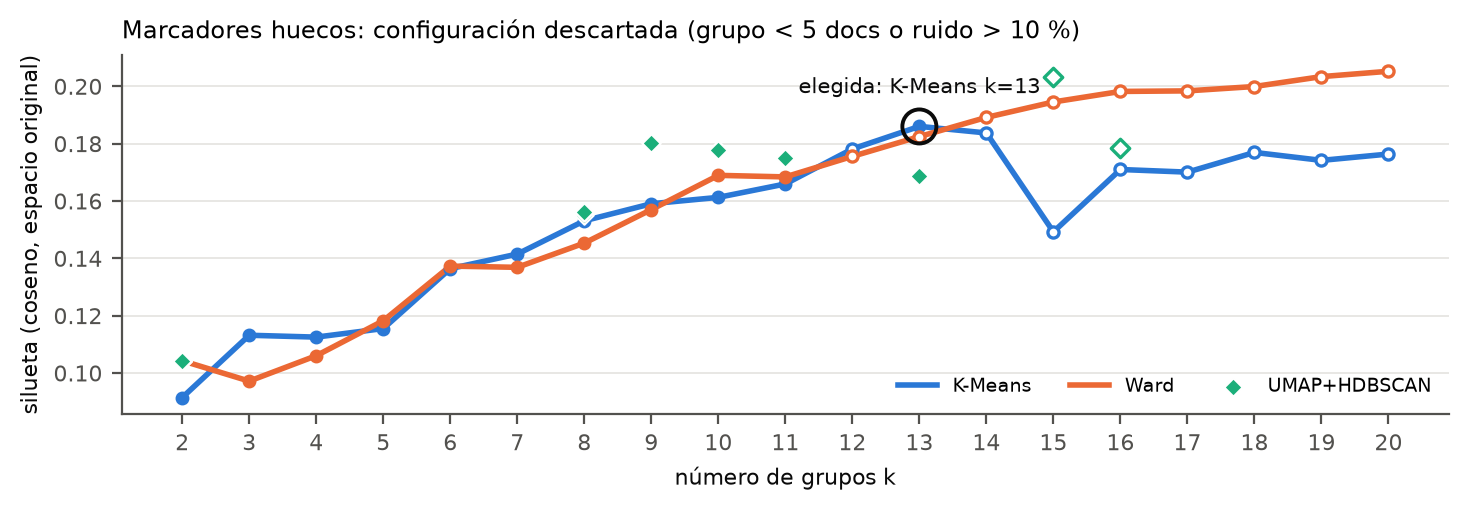
\includegraphics[width=0.84\linewidth]{silueta_estrategias.png}
\caption{Silueta por estrategia y $k$. Ward sigue subiendo hasta $k=20$, pero con grupos de 2 documentos: la
silueta premia la fragmentación, de ahí la restricción de tamaño.}
\end{figure}

\begin{table}[H]
\centering\footnotesize\setlength{\tabcolsep}{5pt}
\begin{tabular}{@{}llcccccc@{}}
\toprule
\textbf{Estrategia} & \textbf{Mejor configuración válida} & $k$ & \textbf{Silueta} & \textbf{DB} & \textbf{Ruido} & \textbf{Grupo mín.} & \textbf{Estabilidad (ARI)} \\
\midrule
K-Means (\texttt{n\_init}=50)  & $k=13$                          & 13 & \textbf{0.186} & \textbf{2.16} & 0\,\%  & 5 & 0.62 $\pm$ 0.07 \\
Aglomerativo Ward              & $k=10$                          & 10 & 0.169 & 2.37 & 0\,\%  & 6 & \textbf{0.74 $\pm$ 0.10} \\
UMAP 5D + HDBSCAN              & \texttt{nn}=10, \texttt{mcs}=6  &  9 & 0.180 & 2.27 & 10\,\% & 8 & 0.46 $\pm$ 0.28 \\
HDBSCAN directo en 768\,d      & \texttt{mcs}=5 (no válida)      &  2 & 0.056 & 1.58 & 82.5\,\% & 5 & --- \\
\bottomrule
\end{tabular}
\end{table}

\textbf{Configuración defendida: K-Means con $k=13$}, que tiene la mayor silueta y el menor DB entre las
válidas. La \emph{alternativa} razonable es Ward con $k=10$, menos separada pero más estable: conviene si se
prefieren menos grupos y reproducibles. UMAP + HDBSCAN es la más frágil: su partición cambia mucho con la
semilla de UMAP ($\pm$0.28). HDBSCAN aplicado directo en 768 dimensiones fracasa, porque las distancias se
concentran y el 82.5\,\% de los documentos queda como ruido; por eso hay que reducir antes. Conviene leer la
silueta en términos absolutos: \textbf{0.19 es baja}. Los documentos son breves y los temas se tocan, y
\textbf{16 de 120 documentos} tienen silueta negativa, es decir, están más cerca de otro grupo que del suyo.

\section{Tópicos: cómo leer cada grupo sin abrir los documentos}

Cada grupo se caracteriza con tres piezas: (a) sus términos \textbf{c-TF-IDF}, que se obtienen concatenando
el grupo y ponderando $\frac{tf_{t,c}}{\lVert tf_c\rVert_1}\log(1+\frac{A}{f_t})$, lo que premia lo
frecuente dentro del grupo y raro fuera de él; (b) una etiqueta con sus 3 primeros términos; y (c) los
documentos más cercanos al centroide. Los términos no llevan \emph{stemming}, porque los lee una persona, y
deben aparecer en al menos 2 documentos del grupo. Frente a dos alternativas más simples, c-TF-IDF da
tópicos más coherentes y menos repetidos. Coherencia NPMI de los 10 primeros términos: \textbf{$-$0.11},
frente a $-$0.35 de la frecuencia bruta y $-$0.31 del TF-IDF medio. Diversidad: \textbf{0.97}, frente a 0.93
y 0.95.

\begin{table}[H]
\centering\footnotesize\setlength{\tabcolsep}{4pt}
\begin{tabular}{@{}rr>{\raggedright\arraybackslash}p{6.0cm}>{\raggedright\arraybackslash}p{5.5cm}r@{}}
\toprule
\textbf{G} & \textbf{Docs} & \textbf{Etiqueta y términos c-TF-IDF} & \textbf{Documentos representativos} & \textbf{Silueta} \\
\midrule
3  & 21 & \textbf{energía · carbono · emisiones}; solar, contaminación, combustión, residuos & Aviación y combustibles sostenibles; Escasez de agua & 0.07 \\
8  & 13 & \textbf{datos · modelo · aprendizaje}; lenguaje, recuperación, visión & MLOps; Modelos de lenguaje y \emph{transformers} & 0.13 \\
2  & 12 & \textbf{temperatura · fermentación · masa}; gluten, cocina, arroz, acidez & El arte de la masa madre; Cocina mexicana y maíz & 0.23 \\
6  & 11 & \textbf{fuerza · física · sueño}; resistencia, cardiovasculares, especialista & Actividad física y longevidad; Salud mental & 0.06 \\
1  & 10 & \textbf{criptografía · clave · confianza}; pública, llaves, factor & Autenticación multifactor; Confianza cero & 0.34 \\
4, 7 & 9, 9 & \textbf{música · musical · espacios} / \textbf{mercado · deuda · inflación} & Música barroca; Impresionismo / Bancos centrales; Inflación & 0.11, 0.26 \\
9  & 8 & \textbf{alta · velocidad · transporte}; ciclismo, bicicleta & Transporte público; Trenes de alta velocidad & 0.21 \\
5, 12 & 6, 5 & \textbf{órbita · luna · marte} / \textbf{estrellas · galaxias · negros} & Misiones tripuladas; Cohetes / Agujeros negros; Materia oscura & 0.21, 0.37 \\
10, 0, 11 & 6, 5, 5 & \textbf{guerra · pueblos} / \textbf{glaciares · alpes} / \textbf{fútbol · saque · equipos} & Peste negra / Patagonia; Islandia / Baloncesto; Tenis & 0.33, 0.26, 0.17 \\
\bottomrule
\end{tabular}
\end{table}

\textbf{Tópicos emergentes.} El método no se limita a reproducir un índice temático; reorganiza el corpus por
\emph{de qué habla} cada texto:
\begin{itemize}
\item \textbf{G3, «energía y clima» (21 docs):} junta Medio Ambiente con los textos de transporte que hablan
de emisiones (coche eléctrico, baterías, aviación sostenible). Es un tópico transversal real, pero también es
el «cajón» de K-Means: absorbe 5 textos de historia y viajes sin hogar claro (la Revolución Industrial, la
Ruta de la Seda, el Amazonas), todos con silueta negativa. Por eso su silueta es de 0.07.
\item \textbf{G6, «salud y actividad física»:} el maratón, la natación y las lesiones se unen con salud, no con
deportes. Los deportes de equipo y su estadística forman otro grupo (G11).
\item \textbf{La astronomía se parte en dos:} exploración espacial (G5: Luna, Marte, cohetes) y astrofísica
(G12: agujeros negros, ondas gravitacionales). G12 es el grupo más compacto del corpus (silueta 0.37).
\end{itemize}

\section{Proyección con UMAP: qué muestra y qué distorsiona}

\textbf{Técnica.} El mapa debe conservar los \emph{vecindarios}, que es lo que el lector inspecciona, y usar la
misma distancia coseno de los grupos. PCA es lineal y con 2 componentes explica solo el 13.7\,\% de la
varianza. t-SNE no conserva la disposición global. Se usó \textbf{UMAP} (\texttt{metric=cosine}) con dos
configuraciones, medidas contra el espacio original y promediadas sobre 5 semillas.

\begin{table}[H]
\centering\footnotesize\setlength{\tabcolsep}{5pt}
\begin{tabular}{@{}lcccc@{}}
\toprule
\textbf{Proyección} & \textbf{\emph{Trustw.}@10} & \textbf{Vecinos pres.@10} & \textbf{Spearman dist.} & \textbf{Silueta 2D} \\
\midrule
UMAP A · local (\texttt{nn}=5, \texttt{md}=0.0) & \textbf{0.921} $\pm$ 0.003 & \textbf{0.644} & 0.408 & 0.512 \\
UMAP B · global (\texttt{nn}=30, \texttt{md}=0.5) & 0.902 $\pm$ 0.011 & 0.602 & \textbf{0.578} & 0.270 \\
PCA (referencia lineal)                                            & 0.805 & 0.398 & 0.532 & 0.012 \\
\bottomrule
\end{tabular}
\end{table}

\begin{figure}[H]
\centering
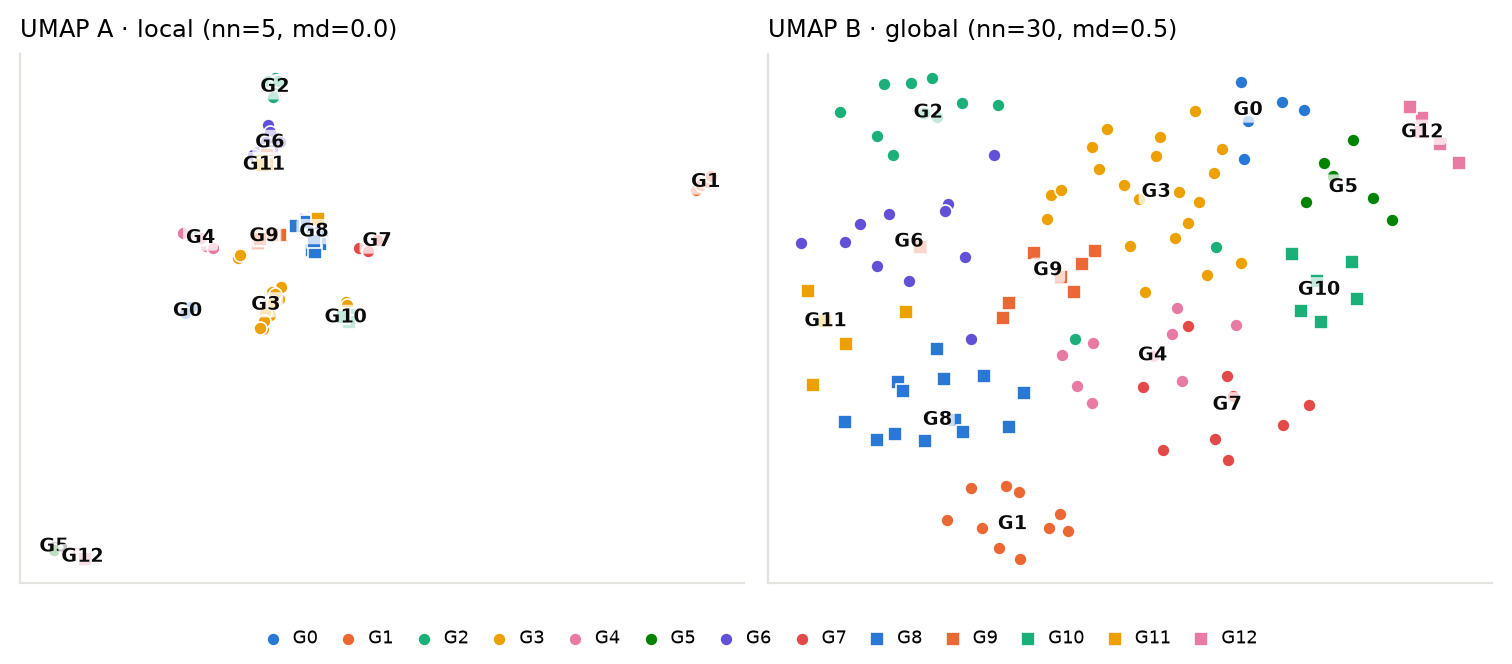
\includegraphics[width=0.92\linewidth]{umap_comparacion.png}
\caption{La misma partición (K-Means, $k=13$) en las dos configuraciones de UMAP. Los grupos no cambian; solo
cambia el dibujo.}
\end{figure}

\textbf{Lo que muestra:} vecindarios fiables. En A, el 92\,\% de los vecinos que se ven en el mapa son vecinos
reales, y en 115 de 120 documentos el punto más cercano en el dibujo está entre sus 10 vecinos reales.
\textbf{Lo que distorsiona:} (1) \textbf{la separación}, porque la silueta pasa de 0.19 en el espacio original
a 0.51 en A: el mapa exagera $2.7\times$ lo bien separados que están los grupos. (2) \textbf{Las distancias
entre grupos}: A arroja la astronomía a una esquina y la ciberseguridad a otra, sin que esa distancia
signifique nada (Spearman 0.41). (3) \textbf{Los tamaños}: \texttt{min\_dist}=0 aplasta cada grupo en un punto
y oculta su dispersión real. (4) Hay \textbf{falsos vecinos}: \emph{Comercio internacional} queda junto a
\emph{Automatización y empleo} (coseno 0.43), aunque su vecino real es \emph{Bancos centrales} (0.72). B
sacrifica algo de precisión local a cambio de mejor disposición global (Spearman 0.58) y de puntos repartidos
que se pueden señalar. Por eso B es la vista por defecto de la interfaz.

\paragraph{Interfaz.} Un \texttt{go.FigureWidget} de plotly, que es un \emph{widget} de \texttt{ipywidgets}, con:
proyección (A, B o PCA); color por grupo o por la categoría oculta; filtro por grupo; resaltado de un
término (p.\,ej. \term{energía} marca 5 documentos de G3 y uno de G12, por «energía oscura»: la misma palabra en dos tópicos); y selección de un documento por lista o por
clic. La ficha del documento muestra su grupo, su tópico, el texto, su silueta y sus \textbf{5 vecinos reales},
que además se marcan en el mapa. Así el lector detecta cuándo la proyección los separó. El mapa se exporta
también a \texttt{figures/mapa\_corpus.html}.

\section{Auditoría externa, conclusiones y limitaciones}

\textbf{Auditoría.} Solo al final se comparó con las 12 categorías ocultas. K-Means con $k=13$ obtiene
\textbf{ARI 0.58 y NMI 0.79}: 6 de los 13 grupos son 100\,\% puros (tabla de contingencia en el notebook) (Ward: 0.59 y 0.77; UMAP + HDBSCAN: 0.59 y 0.78).
Las tres estrategias coinciden en lo esencial. Las discrepancias no son errores del método; son cortes
distintos: el editor clasificó por \emph{sección} y los \emph{embeddings} agrupan por \emph{contenido}
(el coche eléctrico habla de emisiones, el maratón habla de salud).

\textbf{Conclusiones.} (1) La representación correcta depende de la tarea: para agrupar ganan los modelos
simétricos de paráfrasis, no el mejor recuperador. (2) La silueta sirve para \emph{comparar} configuraciones,
pero sola tiende a premiar la fragmentación; necesita una restricción de utilidad y un control de estabilidad.
(3) c-TF-IDF y los documentos representativos vuelven legible cada grupo. (4) El mapa UMAP sirve para
explorar vecindarios, no para medir distancias ni la calidad de los grupos.

\textbf{Limitaciones.} Con 120 documentos breves, la silueta es baja y las diferencias entre configuraciones
cercanas son del orden de su variación entre semillas (K-Means: $\pm$0.01). K-Means obliga a asignar cada
documento, lo que produce un grupo cajón (G3); un modelo de tópicos con asignación difusa lo reflejaría
mejor. La lista de palabras genéricas para los términos se ajustó tras inspeccionar la primera versión,
aunque sin usar etiquetas. Las métricas de UMAP dependen de la semilla, y por eso se promediaron 5. Por
último, la auditoría usa una sola taxonomía editorial, que es una de varias organizaciones válidas.

\end{document}
